% 2009 年安徽卷文科第 20 题：正方形 ABCD 与平行直线 l 构成的六面体 ABCDEF。
% 来源 PDF：普通高考/2009/2009安徽文.pdf，SHA256 83b982d22fd84a0158f909bce3d1f62e1fa228868e7915ded21e7a5ed9774897
% 原页：第 2 页（A3 三栏）第 2 栏中部，印刷页 498。
% 重绘依据：正方形按斜投影画成平行四边形，A 左下、B 右下、C 右上、D 左上；l 为 AB 上方的水平直线，
%   E、F 在 l 上（F 在右、超出正方形右边界）；E′、F′ 在正方形平面内的中线上，
%   EE′、FF′ 画虚线，DC 画虚线（被遮挡）；实线为 AB、BC、AD 与 E、F 到 A、D、B、C 的连线。
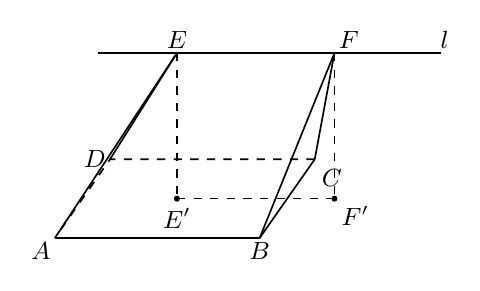
\begin{tikzpicture}[scale=1.0, semithick, every node/.style={inner sep=1.3pt, font=\small}]
  \coordinate (A) at (0,0);
  \coordinate (B) at (2.6,0);
  \coordinate (C) at (3.3,1.0);
  \coordinate (D) at (0.7,1.0);
  \coordinate (E) at (1.55,2.35);
  \coordinate (F) at (3.55,2.35);
  \coordinate (Ep) at (1.55,0.5);
  \coordinate (Fp) at (3.55,0.5);
  % 直线 l
  \draw (0.55,2.35) -- (4.9,2.35);
  \node[above] at (4.95,2.35) {$l$};
  % 正方形
  \draw (A) -- (B) -- (C);
  \draw[dashed] (C) -- (D) -- (A);
  % 棱
  \draw (A) -- (E);
  \draw (D) -- (E);
  \draw (B) -- (F);
  \draw (C) -- (F);
  \draw (E) -- (F);
  % 垂线
  \draw[dashed] (E) -- (Ep);
  \draw[dashed] (F) -- (Fp);
  % 中线
  \draw[dashed] (Ep) -- (Fp);
  \fill (Ep) circle (1.1pt);
  \fill (Fp) circle (1.1pt);
  \node[below left] at (A) {$A$};
  \node[below] at (B) {$B$};
  \node[anchor=north west] at ([xshift=1pt,yshift=-2pt]C) {$C$};
  \node[left] at (D) {$D$};
  \node[above] at (E) {$E$};
  \node[anchor=south west] at (F) {$F$};
  \node[below] at ([yshift=-2pt]Ep) {$E'$};
  \node[anchor=north west] at ([xshift=1pt,yshift=-1pt]Fp) {$F'$};
\end{tikzpicture}
